% !TeX program = xelatex
\documentclass[a4paper,10pt]{article}

% ============================================================================
% កញ្ចប់បណ្ណាល័យ (Packages) – តាមលំនាំ NGS Preah Krasang (ls_plan.tex)
% បរិបទ៖ គ្មានស្លាយ LCD និងគ្មានម៉ាស៊ីនគិតលេខ — ប្រើសន្លឹកកិច្ចការសិស្ស (ស-ខ្មៅ) និងក្ដារខៀនជាគោល
% ============================================================================
\usepackage[a4paper, left=0.95cm, right=0.95cm, top=0.85cm, bottom=0.92cm, footskip=0.52cm]{geometry}
\usepackage{amsmath}
\usepackage{unicode-math}
\usepackage{fontspec}
\usepackage{array, longtable, multirow, colortbl}
\usepackage[table]{xcolor}
\usepackage{enumitem}
\usepackage{pifont}
\usepackage{fancyhdr}
\usepackage{tikz}
\usetikzlibrary{calc, arrows.meta, angles, quotes, decorations.markings, decorations.pathreplacing, patterns, babel}

\makeatletter
\let\@expl@@@mark@update@singlecol@structures@@\relax
\makeatother

\providecommand{\NGSFindFonts}{%
  \IfFileExists{C:/Windows/Fonts/cambria.ttc}{%
    \def\NGSSysPath{C:/Windows/Fonts/}%
    \def\NGSUserPath{C:/Users/KIT/AppData/Local/Microsoft/Windows/Fonts/}%
  }{%
    \IfFileExists{./fonts/KhmerOSsiemreap.ttf}{\def\NGSSysPath{./fonts/}\def\NGSUserPath{./fonts/}}{%
    \IfFileExists{../fonts/KhmerOSsiemreap.ttf}{\def\NGSSysPath{../fonts/}\def\NGSUserPath{../fonts/}}{%
    \IfFileExists{../../fonts/KhmerOSsiemreap.ttf}{\def\NGSSysPath{../../fonts/}\def\NGSUserPath{../../fonts/}}{%
    \IfFileExists{../../../fonts/KhmerOSsiemreap.ttf}{\def\NGSSysPath{../../../fonts/}\def\NGSUserPath{../../../fonts/}}{%
    \IfFileExists{../../../../fonts/KhmerOSsiemreap.ttf}{\def\NGSSysPath{../../../../fonts/}\def\NGSUserPath{../../../../fonts/}}{%
    \IfFileExists{../../../../../fonts/KhmerOSsiemreap.ttf}{\def\NGSSysPath{../../../../../fonts/}\def\NGSUserPath{../../../../../fonts/}}{%
    \IfFileExists{../../../../../../fonts/KhmerOSsiemreap.ttf}{\def\NGSSysPath{../../../../../../fonts/}\def\NGSUserPath{../../../../../../fonts/}}{%
      \def\NGSSysPath{../../../../../../../fonts/}\def\NGSUserPath{../../../../../../../fonts/}%
    }}}}}}}%
  }%
}
\NGSFindFonts

\setmathfont[Path={\NGSSysPath}, FontIndex=1, Scale=1.02]{cambria.ttc}
\defaultfontfeatures{Ligatures=TeX}

\setmainfont[
  Path={\NGSUserPath}, Extension=.ttf, Script=Khmer,
  BoldFont={KhmerOSsiemreap}, BoldFeatures={FakeBold=1.8},
  ItalicFont={KhmerOSsiemreap}, ItalicFeatures={FakeSlant=0.25},
  BoldItalicFont={KhmerOSsiemreap}, BoldItalicFeatures={FakeBold=1.8, FakeSlant=0.25}
]{KhmerOSsiemreap}

\newfontfamily\muol[Path={\NGSUserPath}, Extension=.ttf, Script=Khmer]{KhmerOSmuollight}
\newfontfamily\TimesEn[Path={\NGSSysPath}, Extension=.ttf, Scale=1.00, BoldFont={timesbd}, ItalicFont={timesi}, BoldItalicFont={timesbi}]{times}
\newfontfamily\NagaBold[Path={\NGSUserPath}, Extension=.ttf]{AKbalthom Naga Bold}
\newfontfamily\CalibriFont[Path={\NGSSysPath}, Extension=.ttf]{calibri}
\newfontfamily\Tacteing[Path={\NGSUserPath}]{TACTENG.TTF}
\newfontfamily\CourierBullet[Path={\NGSSysPath}, Extension=.ttf]{cour}
\newcommand{\wcirc}{{\CourierBullet\fontsize{9.5pt}{11pt}\selectfont o}}

\XeTeXlinebreaklocale "km"
\XeTeXlinebreakskip = 0pt plus 1pt minus 0.1pt

\definecolor{stepgray}{HTML}{D9D9D9}
\definecolor{headgray}{HTML}{F2F2F2}
\definecolor{boxgray}{HTML}{D9D9D9}
\definecolor{darkred}{HTML}{C00000}
\definecolor{red5e}{HTML}{FF0000}

\pagestyle{fancy}
\fancyhf{}
\renewcommand{\headrulewidth}{0pt}
\fancyfoot[R]{\CalibriFont\fontsize{11pt}{13pt}\selectfont\thepage}

\setlength{\parindent}{0pt}
\setlength{\parskip}{0pt}
\setlength{\tabcolsep}{3.8pt}

\newcolumntype{L}[1]{>{\raggedright\arraybackslash}p{#1}}
\newcolumntype{C}[1]{>{\centering\arraybackslash}p{#1}}

\newcommand{\en}[1]{{\TimesEn #1}}
\newcommand{\enbf}[1]{{\TimesEn\textbf{#1}}}
\newcommand{\unit}[1]{\,\text{\en{#1}}}
\newcommand{\fiveE}[1]{{\NagaBold\fontsize{9.5pt}{13pt}\selectfont\textcolor{red5e}{#1}}}
\newcommand{\timenote}[1]{\textcolor{darkred}{\textit{#1}}}
\newcommand{\redsub}[1]{\textcolor{darkred}{#1}}
\newcommand{\graybox}[1]{\colorbox{boxgray}{\strut\hspace{2pt}#1\hspace{2pt}}}
\newcommand{\ditem}{\tikz[baseline=-0.5ex]\fill (0,0.42ex) -- (0.42ex,0) -- (0,-0.42ex) -- (-0.42ex,0) -- cycle;\hspace{0.3em}}
\newcommand{\cnum}[1]{{\fontsize{10.5pt}{12pt}\selectfont\ding{\numexpr181+#1\relax}}\hspace{0.15em}}
\newcommand{\cfig}[1]{\par\vspace{3pt}{\centering #1\par}\vspace{3pt}}
\newcommand{\stepheader}[1]{\multicolumn{3}{|c|}{\cellcolor{stepgray}\muol #1} \\* \noalign{\hrule height 0.4pt}}
\newcommand{\khmflourish}{{\Tacteing\fontsize{36pt}{14pt}\selectfont\raisebox{-5pt}{3}}}

% ============================================================================
% ម៉ាក្រូគូសរូប TikZ ស-ខ្មៅ ១០០% សម្រាប់មេរៀន ២.៤.៥ ទម្រង់ស្តង់ដានៃស្វ័យគុណ (STDFORM)
% ============================================================================

% ១. E1 Engage: ល្បឿនពន្លឺ ទល់នឹង កាំអាតូម (ទំ.២១)
\newcommand{\figEngageSTD}{%
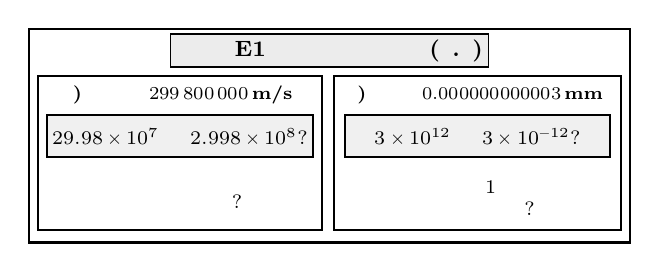
\begin{tikzpicture}[x=0.96cm, y=0.92cm, every node/.style={font=\scriptsize, text=black}]
  \draw[black, line width=0.95pt] (0,0) rectangle (7.95,2.95);
  \node[fill=gray!15, draw=black, line width=0.6pt, inner sep=2pt, font=\footnotesize\bfseries] at (3.975,2.65) {បេសកកម្ម \en{E1}៖ ល្បឿនពន្លឺ និងកាំអាតូម (ទំ.២១)};

  \draw[black, line width=0.8pt] (0.12,0.18) rectangle (3.88,2.30);
  \node[font=\fontsize{6.6pt}{8.5pt}\selectfont\bfseries] at (2.00,2.04) {១) ល្បឿនពន្លឺ $299\,800\,000\unit{m/s}$};
  \draw[black, line width=0.75pt, fill=gray!12] (0.24,1.18) rectangle (3.76,1.76);
  \node at (2.00,1.47) {$29.98\times 10^7$ \;ឬ\; $2.998\times 10^8$?};
  \node[align=center] at (2.00,0.62) {តើទម្រង់មួយណាជា\\\textbf{ទម្រង់ស្តង់ដាផ្លូវការ}?};

  \draw[black, line width=0.8pt] (4.04,0.18) rectangle (7.83,2.30);
  \node[font=\fontsize{6.5pt}{8.5pt}\selectfont\bfseries] at (5.935,2.04) {២) កាំអាតូម $0.000000000003\unit{mm}$};
  \draw[black, line width=0.75pt, fill=gray!12] (4.18,1.18) rectangle (7.69,1.76);
  \node at (5.935,1.47) {$3\times 10^{12}$ \;ឬ\; $3\times 10^{-12}$?};
  \node[align=center] at (5.935,0.62) {តើចំនួនតូចជាង $1$ ត្រូវមាន\\និទស្សន្ត \textbf{បូក} ឬ \textbf{ដក}?};
\end{tikzpicture}}

% ២. E2 POE 1 & 2: ច្រកទ្វារមេគុណ 1 <= A < 10 និងយុថ្កាទំហំធំ-តូច
\newcommand{\figGateSTD}{%
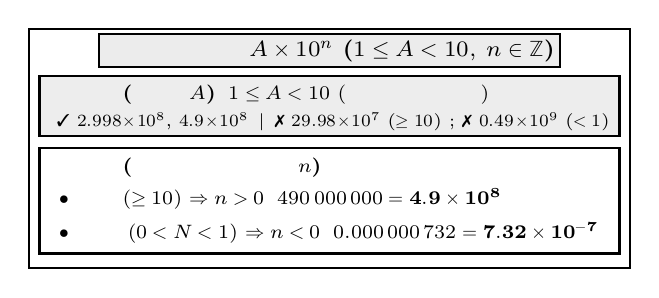
\begin{tikzpicture}[x=0.96cm, y=0.92cm, every node/.style={font=\scriptsize, text=black}]
  \draw[black, line width=0.95pt] (0,0) rectangle (7.95,3.30);
  \node[fill=gray!15, draw=black, line width=0.6pt, inner sep=2pt, font=\footnotesize\bfseries] at (3.975,3.00) {ច្រកទ្វារទម្រង់ស្តង់ដា $A\times 10^n$ ($1\le A < 10,\; n\in\mathbb{Z}$)};

  % Gate box
  \draw[black, line width=0.9pt, fill=gray!14] (0.14,1.82) rectangle (7.81,2.65);
  \node[anchor=west] at (0.24,2.40) {\textbf{លក្ខខណ្ឌ ១ (ច្រកមេគុណ $A$)៖} $1\le A < 10$ (មុខក្បៀស ១ ខ្ទង់មិនសូន្យ)};
  \node[anchor=west, font=\fontsize{6.2pt}{8pt}\selectfont] at (0.24,2.02) {\ding{51} $2.998\!\times\! 10^8$, $4.9\!\times\! 10^8$ \,\textbar\, \ding{55} $29.98\!\times\! 10^7$ ($\ge 10$) ; \ding{55} $0.49\!\times\! 10^9$ ($<1$)};

  % Magnitude anchor
  \draw[black, line width=0.85pt] (0.14,0.20) rectangle (7.81,1.66);
  \node[anchor=west] at (0.24,1.38) {\textbf{លក្ខខណ្ឌ ២ (យុថ្កាទំហំកំណត់សញ្ញានិទស្សន្ត $n$)៖}};
  \node[anchor=west] at (0.28,0.96) {$\bullet$ ចំនួនធំ ($\ge 10$) $\Rightarrow n > 0$៖ $490\,000\,000 = \mathbf{4.9\times 10^8}$};
  \node[anchor=west] at (0.28,0.48) {$\bullet$ ចំនួនតូច ($0<N<1$) $\Rightarrow n < 0$៖ $0.000\,000\,732 = \mathbf{7.32\times 10^{-7}}$};
\end{tikzpicture}}

% ៣. E4 Worked Example 2: ប្រៀបធៀបអង្កត់ផ្ចិតភពព្រហស្បតិ៍ និងផែនដី (ទំ.២១-២២)
\newcommand{\figJupiterSTD}{%
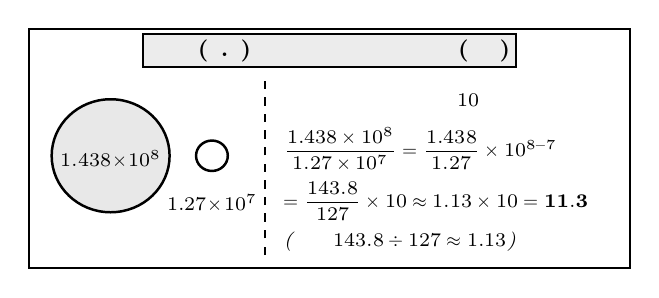
\begin{tikzpicture}[x=0.96cm, y=0.92cm, every node/.style={font=\scriptsize, text=black}]
  \draw[black, line width=0.95pt] (0,0) rectangle (7.95,3.30);
  \node[fill=gray!15, draw=black, line width=0.6pt, inner sep=2pt, font=\footnotesize\bfseries] at (3.975,3.00) {គំរូ ២ (ទំ.២១)៖ ប្រៀបធៀបភពព្រហស្បតិ៍ និងផែនដី (ចែកដៃ)};

  % Left circles
  \draw[black, line width=0.9pt, fill=gray!18] (1.08,1.55) circle (0.78);
  \node[align=center] at (1.08,1.55) {\textbf{ព្រហស្បតិ៍}\\$1.438\!\times\! 10^8$};
  \draw[black, line width=0.9pt, fill=white] (2.42,1.55) circle (0.21);
  \node[align=center] at (2.42,0.95) {\textbf{ផែនដី}\\$1.27\!\times\! 10^7$};

  \draw[black, dashed, line width=0.6pt] (3.12,0.18) -- (3.12,2.68);

  % Right calculation
  \node[anchor=west] at (3.24,2.32) {\textbf{ផ្ដុំមេគុណ ចែកដាច់ពីស្វ័យគុណនៃ $10$៖}};
  \node[anchor=west] at (3.24,1.65) {$\dfrac{1.438\times 10^8}{1.27\times 10^7} = \dfrac{1.438}{1.27}\times 10^{8-7}$};
  \node[anchor=west] at (3.24,0.92) {$= \dfrac{143.8}{127}\times 10 \approx 1.13\times 10 = \mathbf{11.3\text{ ដង}}$};
  \node[anchor=west] at (3.24,0.36) {\textit{(ចែកដៃ៖ $143.8\div 127 \approx 1.13$)}};
\end{tikzpicture}}

% ៤. E5 Diagnostic Options A-D
\newcommand{\figExitCardsSTD}{%
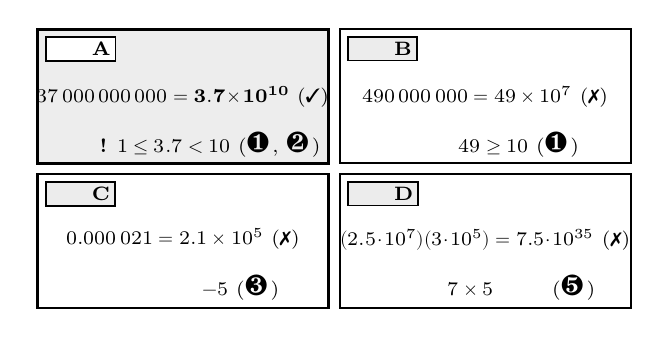
\begin{tikzpicture}[x=0.96cm, y=0.92cm, every node/.style={font=\scriptsize, text=black}]
  \draw[black, line width=1.1pt, fill=gray!14] (0,2.00) rectangle (3.85,3.85);
  \node[anchor=north west, fill=white, draw=black, line width=0.6pt, inner sep=1.8pt] at (0.10,3.75) {\textbf{ជម្រើស \en{A}}};
  \node at (1.925,2.92) {$37\,000\,000\,000 = \mathbf{3.7\!\times\! 10^{10}}$ (\ding{51})};
  \node at (1.925,2.25) {\textbf{ត្រឹមត្រូវ!} $1\le 3.7<10$ (\cnum{1}, \cnum{2})};

  \draw[black, line width=0.9pt] (4.00,2.00) rectangle (7.85,3.85);
  \node[anchor=north west, fill=gray!15, draw=black, line width=0.6pt, inner sep=1.8pt] at (4.10,3.75) {\textbf{ជម្រើស \en{B}}};
  \node at (5.925,2.92) {$490\,000\,000 = 49\times 10^7$ (\ding{55})};
  \node at (5.925,2.25) {ខុសលក្ខខណ្ឌ $49 \ge 10$ (\cnum{1})};

  \draw[black, line width=0.9pt] (0,0) rectangle (3.85,1.85);
  \node[anchor=north west, fill=gray!15, draw=black, line width=0.6pt, inner sep=1.8pt] at (0.10,1.75) {\textbf{ជម្រើស \en{C}}};
  \node at (1.925,0.95) {$0.000\,021 = 2.1\times 10^{5}$ (\ding{55})};
  \node at (1.925,0.28) {ភ្លេចដាក់និទស្សន្តដក $-5$ (\cnum{3})};

  \draw[black, line width=0.9pt] (4.00,0) rectangle (7.85,1.85);
  \node[anchor=north west, fill=gray!15, draw=black, line width=0.6pt, inner sep=1.8pt] at (4.10,1.75) {\textbf{ជម្រើស \en{D}}};
  \node at (5.925,0.95) {$(2.5\!\cdot\! 10^7)(3\!\cdot\! 10^5) = 7.5\!\cdot\! 10^{35}$ (\ding{55})};
  \node at (5.925,0.28) {គុណនិទស្សន្ត $7\times 5$ ជំនួសបូក (\cnum{5})};
\end{tikzpicture}}

\begin{document}
\fontsize{10pt}{15.2pt}\selectfont

% -------------------- ក្បាលកិច្ចតែងការ --------------------
\begin{center}
  {\muol\fontsize{11pt}{16pt}\selectfont ព្រះរាជាណាចក្រកម្ពុជា}\\[2pt]
  {\muol\fontsize{10pt}{15pt}\selectfont ជាតិ សាសនា ព្រះមហាក្សត្រ}\\[1pt]
  \khmflourish
\end{center}

\vspace{-24pt}
{\muol\fontsize{9.5pt}{12.5pt}\selectfont
មន្ទីរអប់រំ យុវជន និងកីឡា ខេត្តកំពង់ធំ\\
ការិយាល័យអប់រំ យុវជន និងកីឡា ស្រុកកំពង់ស្វាយ\\
អនុវិទ្យាល័យព្រះក្រសាំង}

\vspace{1pt}
\begin{center}
  {\muol\fontsize{10pt}{14pt}\selectfont កិច្ចតែងការបង្រៀន}
\end{center}
\vspace{0pt}

% -------------------- ព័ត៌មានទូទៅ --------------------
{\renewcommand{\arraystretch}{0.98}
\hspace*{3.1cm}%
\begin{tabular}{@{}l l L{11.0cm}@{}}
  - \hspace{0.35cm} មុខវិជ្ជា & : & គណិតវិទ្យា ថ្នាក់ទី៨ (ពីជគណិត) \\
  - \hspace{0.35cm} ចំណងជើងមេរៀន & : & មេរៀនទី២៖ ស្វ័យគុណ \\
  - \hspace{0.35cm} ចំណងជើងរង & : & ៤.៥. ទម្រង់ស្តង់ដានៃស្វ័យគុណ (សៀវភៅពុម្ព ទំ.២១–២២ និងលំហាត់ \#9, \#11 ទំ.២៦) \\
  - \hspace{0.35cm} រយៈពេល & : & ១ ម៉ោងសិក្សា (៥០ នាទី) \\
  - \hspace{0.35cm} បង្រៀនដោយ & : & ហុក ប៊ុនថែន \\
  - \hspace{0.35cm} កាលបរិច្ឆេទ & : & ថ្ងៃពុធ ទី១៨ ខែវិច្ឆិកា ឆ្នាំ២០២៦ \\
\end{tabular}

\vspace{2pt}

% -------------------- I. វត្ថុបំណង --------------------
\textbf{I.} {\muol វត្ថុបំណង}\\[1pt]
\hspace*{0.55cm}%
\begin{tabular}{@{}l l L{14.2cm}@{}}
  \wcirc \hspace{0.25cm} វិជ្ជាសម្បទា & : & សិស្សប្រាប់និយមន័យទម្រង់ស្តង់ដានៃស្វ័យគុណ $A\times 10^n$ ដែល $1\le A < 10$ ហើយ $n$ ជាចំនួនគត់រ៉ឺឡាទីប ($n\in\mathbb{Z}$) ព្រមទាំងកំណត់សញ្ញានៃនិទស្សន្ត $n$ តាមទំហំចំនួនធំ ($\ge 10$) ឬតូច ($0<N<1$) ។ \\
  \wcirc \hspace{0.25cm} បំណិនសម្បទា & : & សិស្សសរសេរចំនួនធំណាស់ និងតូចណាស់ក្នុងទម្រង់ស្តង់ដា ព្រមទាំងគណនាផលគុណ និងផលធៀបនៃចំនួនក្នុងទម្រង់ស្តង់ដា (ទំ.២១–២២ និង ទំ.២៦ \#9, \#11) លើសន្លឹកកិច្ចការដោយមិនប្រើម៉ាស៊ីនគិតលេខ ។ \\
  \wcirc \hspace{0.25cm} ចរិយាសម្បទា & : & សិស្សមានភាពហ្មត់ចត់ក្នុងការត្រួតពិនិត្យលក្ខខណ្ឌ $1\le A < 10$ និងមានចំណាប់អារម្មណ៍លើការប្រើស្វ័យគុណនៃ $10$ ក្នុងតារាសាស្ត្រ និងរូបវិទ្យា ។ \\
\end{tabular}

\vspace{2pt}

% -------------------- II. សម្ភារៈឧបទេស --------------------
\textbf{II.} {\muol សម្ភារៈឧបទេស}\\[1pt]
\hspace*{0.55cm}$\bullet$ \hspace{0.35cm} សៀវភៅសិក្សាគោលគណិតវិទ្យាថ្នាក់ទី៨ (ទំ.២១–២២, ២៦) ក្ដារខៀន ដីស និងសន្លឹកកិច្ចការសិស្ស ស-ខ្មៅ (\en{Worksheet\_STDFORM} ទំព័រ ១–២ សម្រាប់បំពេញផ្ទាល់ គ្មានស្លាយ \en{LCD})

\vspace{2pt}

% -------------------- III. វិធីសាស្រ្តបង្រៀន --------------------
\textbf{III.} {\muol វិធីសាស្រ្តបង្រៀន}\\[1pt]
\hspace*{0.45cm}%
\begin{tabular}{@{}l l L{14.85cm}@{}}
  $\bullet$ \hspace{0.25cm} គោលវិធី & : & សិស្សមជ្ឈមណ្ឌល (បង្រៀនតាមសន្លឹកកិច្ចការស៊ើបអង្កេត និងក្ដារខៀន គ្មាន \en{LCD}) \\
  $\bullet$ \hspace{0.25cm} យុទ្ធវិធីបង្រៀន & : & គំរូ \en{5Es} រួមបញ្ចូលច្រកទ្វារមេគុណ $1\le A < 10$ (\en{Coefficient Gate}), យុថ្កាទំហំធំ-តូច (\en{Magnitude Anchor}), និងការផ្ដុំមេគុណ-ស្វ័យគុណសម្រាប់ផលធៀបភព \\
\end{tabular}
}

\vspace{2pt}

% -------------------- IV. ដំណើរការបង្រៀន --------------------
\textbf{IV.} {\muol ដំណើរការបង្រៀន}

\vspace{1pt}

\renewcommand{\arraystretch}{1.15}
\begin{longtable}{|L{5.50cm}|L{7.90cm}|L{4.80cm}|}
\hline
\rowcolor{headgray}
\multicolumn{1}{|c|}{\muol សកម្មភាពគ្រូ} &
\multicolumn{1}{c|}{\muol ខ្លឹមសារមេរៀន} &
\multicolumn{1}{c|}{\muol សកម្មភាពសិស្ស} \\
\hline
\endfirsthead
\hline
\endhead
\hline
\endfoot
\hline
\endlastfoot

% ==================== ជំហានទី១ (2min) ====================
\stepheader{ជំហានទី១ \enbf{(}រដ្ឋបាលថ្នាក់\enbf{)}}
$\bullet$ ពិនិត្យអវត្តមាន អនាម័យ និងសណ្ដាប់ធ្នាប់ថ្នាក់រៀន
&
$\bullet$ រដ្ឋបាលថ្នាក់ និងការរៀបចំដៃគូសិក្សា
&
$\circ$ ប្រធានថ្នាក់រាយការណ៍អវត្តមាន \\[3pt]

$\bullet$ ចែក \textbf{សន្លឹកកិច្ចការសិស្ស (\en{Worksheet\_STDFORM})} ម្នាក់ ១ សន្លឹក (ផ្កាប់ទុកសិន)
&
$\bullet$ សន្លឹកកិច្ចការសិស្ស ស-ខ្មៅ (\en{Worksheet\_STDFORM} ទំព័រ ១–២)
&
$\circ$ ទទួលសន្លឹកកិច្ចការ និងត្រៀមសម្ភារៈសរសេរ \\
\hline

% ==================== ជំហានទី២ (9min: <=3 + 3 + E1 3) ====================
\stepheader{ជំហានទី២ \enbf{(}កិច្ចការផ្ទះ \enbf{+} ទំនាក់ទំនងមេរៀនថ្មី\enbf{)}}
\ditem \textbf{កំណែកិច្ចការផ្ទះ ($\le 3\unit{min}$)} \timenote{(កុំសរសេរវែង)} \par
$\bullet$ ហៅសិស្ស ២ នាក់ឡើងសរសេរចម្លើយលំហាត់ \#10 (ទំ.២៦ — ប្ដូរ $\unit{ml}\to\unit{l}$) លើក្ដារខៀន
&
{\centering\redsub{កំណែកិច្ចការផ្ទះមេរៀន ៤.៤ (ទំ.២៦ \#10)}\par} \par
$\bullet$ $330\unit{ml} = \dfrac{33}{100}\unit{l} = 0.33\unit{l}$ \; ; \; $1365\unit{ml} = \dfrac{273}{200}\unit{l} = 1.365\unit{l}$ \par
$\bullet$ $3800\unit{ml} = \dfrac{19}{5}\unit{l} = 3.8\unit{l}$ \; ; \; $17500\unit{ml} = \dfrac{35}{2}\unit{l} = 17.5\unit{l}$
&
$\circ$ ផ្ទៀងផ្ទាត់ចម្លើយក្នុងតារាងកិច្ចការផ្ទះ \\[3pt]

\ditem \textbf{រំលឹកមេរៀនទាក់ទង (3min)} \par
$\bullet$ ឱ្យសិស្សគណនារហ័ស៖ $4.9 \times 10^8$ និង $7.32 \times 10^{-4}$ ជាចំនួនធម្មតា
&
{\centering\redsub{រំលឹកការរំកិលក្បៀស និងច្បាប់ $\frac{10^m}{10^n}$}\par} \par
$\bullet$ $4.9 \times 10^8 = 490\,000\,000$ \; ; \; $7.32 \times 10^{-4} = 0.000732$ \par
$\bullet$ $\dfrac{10^8}{10^7} = 10^{8-7} = 10^1 = 10$ \;និង\; $10^7\times 10^5 = 10^{12}$
&
$\circ$ ឆ្លើយរហ័សអំពីការរំកិលក្បៀស និងច្បាប់ស្វ័យគុណ \\[3pt]

\fiveE{E1 - Engage (3min)} \timenote{(កុំទាន់ផ្ដល់ចម្លើយ)} \par
\ditem \textbf{«បេសកកម្មអវកាស និងអាតូម៖ ល្បឿនពន្លឺ និងកាំអាតូម» (ទំ.២១)} \par
$\bullet$ ឱ្យសិស្សបើកសន្លឹកកិច្ចការទំព័រ ១ គូសធីកទស្សន៍ទាយលើសំណួរ ២
&
{\centering\redsub{បេសកកម្ម E1៖ ល្បឿនពន្លឺ និងកាំអាតូម (ទំ.២១)}\par} \par
$\bullet$ \textbf{សំណួរ ១៖} ល្បឿនពន្លឺ $299\,800\,000\unit{m/s}$ — តើ $29.98\times 10^7$ ឬ $2.998\times 10^8$ ជាទម្រង់ស្តង់ដាផ្លូវការ? \par
$\bullet$ \textbf{សំណួរ ២៖} កាំអាតូម $0.000\,000\,000\,003\unit{mm}$ — ស្មើ $3\times 10^{12}$ ឬ $3\times 10^{-12}$?
&
$\circ$ គូសធីកទស្សន៍ទាយលើសន្លឹកកិច្ចការទំព័រ ១ \\[3pt]

&
\cfig{\figEngageSTD}
& \\[3pt]

$\bullet$ ស្រង់ចំនួនដៃសិស្សកត់លើក្ដារខៀន (មិនទាន់ប្រាប់ចម្លើយត្រូវ)
&
$\bullet$ ស្ថិតិទស្សន៍ទាយ៖ $29.98\times 10^7$ ទល់នឹង $2.998\times 10^8$ ; $10^{12}$ ទល់នឹង $10^{-12}$
&
$\circ$ លើកដៃបង្ហាញការទស្សន៍ទាយ \\
\hline

% ==================== ជំហានទី៣ (17min: E2 11m + E3 6m) ====================
\stepheader{ជំហានទី៣ \enbf{(}ខ្លឹមសារមេរៀនថ្មី\enbf{)}}
\fiveE{E2 - Explore (11min)} \par
$\bullet$ សរសេរចំណងជើងរងលើក្ដារខៀន
&
\textbf{៤.៥. ទម្រង់ស្តង់ដានៃស្វ័យគុណ} (សៀវភៅពុម្ព ទំ.២១–២២)
&
$\circ$ កត់ចំណងជើងចូលសៀវភៅ \\[3pt]

\ditem \textbf{សកម្មភាព ១៖ ច្រកទ្វារមេគុណ $1\le A < 10$ \en{POE 1} (6min, ផ្នែកទី១-ក)} \par
$\bullet$ ឱ្យដៃគូពិនិត្យតារាងបំបែក $299\,800\,000$ ជា ៣ របៀបលើសន្លឹកកិច្ចការ ហើយផ្ទៀងនឹងឧទាហរណ៍សៀវភៅពុម្ព ទំ.២១
&
{\centering\textbf{សកម្មភាព ១ (\en{POE 1})៖ ច្រកទ្វារមេគុណ $1\le A < 10$}\par} \par
$\bullet$ $2998\times 10^5$ ($A=2998 \ge 10$ \ding{55}) ; \; $29.98\times 10^7$ ($A=29.98 \ge 10$ \ding{55}) \par
$\bullet$ $\mathbf{2.998\times 10^8}$ ($1 \le 2.998 < 10$ \ding{51} — មុខក្បៀសមានលេខមិនសូន្យតែ $1$ ខ្ទង់!)
&
$\circ$ ពិនិត្យតម្លៃ $A$ ក្នុងតារាង \en{POE 1} និងគូសធីកទម្រង់ដែលឆ្លងផុតច្រកទ្វារ $1\le A < 10$ \\[3pt]

\ditem \textbf{សកម្មភាព ២៖ យុថ្កាទំហំកំណត់សញ្ញានិទស្សន្ត $n$ \en{POE 2} (5min, ផ្នែកទី១-ខ)} \par
$\bullet$ ឱ្យដៃគូប្រៀបធៀបចំនួនធំ $299\,800\,000$ និងចំនួនតូច $0.000\,000\,000\,003$ (ទំ.២១)
&
{\centering\textbf{សកម្មភាព ២ (\en{POE 2})៖ យុថ្កាទំហំធំ ($\ge 10$) និងតូច ($<1$)}\par} \par
$\bullet$ $299\,800\,000 \ge 10 \implies$ ក្បៀសស្ដាំ $2$ ត្រូវគុណនឹង $10^8 \implies \mathbf{2.998\times 10^8}$ ($n=+8$) \par
$\bullet$ $0.000\,000\,000\,003 < 1 \implies 3 \times \dfrac{1}{10^{12}} = \mathbf{3\times 10^{-12}}$ ($n=-12$)
&
$\circ$ រាប់ចំនួនខ្ទង់រវាងទីតាំងក្បៀសដើម និងទីតាំងក្បៀសថ្មី ព្រមទាំងកំណត់សញ្ញា $n$ \\[3pt]

&
\cfig{\figGateSTD}
& \\[3pt]

% --- E3 Explain (6min) ---
\fiveE{E3 - Explain (6min)} \par
\ditem \textbf{បង្គុំនិយមន័យ «ជាទូទៅ» (ទំ.២១) និងធនាគារហេតុផល (ផ្នែកទី២)} \par
$\bullet$ ឱ្យសិស្សបង្គុំប្រអប់ \textbf{ជាទូទៅ (ទំ.២១)} និងបញ្ជាក់ពាក្យខ្វះលើប្រអប់ទំ.១៣ («ហើយ $n$ ជាចំនួនគត់រ៉ឺឡាទីប»)
&
$\bullet$ \textbf{ជាទូទៅ (ទំ.២១)៖} ទម្រង់ស្តង់ដានៃស្វ័យគុណ សរសេរក្នុងទម្រង់៖ \par
{\centering\graybox{$A \times 10^n$ \quad ($1 \le A < 10$ ហើយ $n \in \mathbb{Z}$)}\par}
$\bullet$ ដែល $n$ ជាចំនួនគត់រ៉ឺឡាទីប \timenote{(បំពេញពាក្យ «ហើយ $n$» ដែលខ្វះលើប្រអប់ទំ.១៣)} ។
&
$\circ$ បំពេញប្រអប់ «ជាទូទៅ» លើសន្លឹកកិច្ចការ និងកត់ចំណាំលើសៀវភៅពុម្ព \\[3pt]

$\bullet$ សង្ខេប \textbf{ធនាគារហេតុផល \cnum{1}--\cnum{5}} សម្រាប់បម្លែង និងគណនាទម្រង់ស្តង់ដា
&
\textbf{ធនាគារហេតុផល \en{B\&W} (\cnum{1}--\cnum{5})៖} \par
\cnum{1} ច្រកទ្វារមេគុណ៖ $1 \le A < 10$ (មុខក្បៀសមានលេខខុសពីសូន្យតែ $1$ ខ្ទង់គត់) \par
\cnum{2} យុថ្កាចំនួនធំ ($N \ge 10$)៖ និទស្សន្តវិជ្ជមាន $n > 0$ ($+$) \par
\cnum{3} យុថ្កាចំនួនតូច ($0 < N < 1$)៖ និទស្សន្តអវិជ្ជមាន $n < 0$ ($-$) \par
\cnum{4} ប្រមាណវិធីគុណ៖ $(A_1\times 10^m)(A_2\times 10^n) = (A_1 A_2)\times 10^{m+n}$ \par
\cnum{5} ប្រមាណវិធីចែក៖ $\dfrac{A_1\times 10^m}{A_2\times 10^n} = \left(\dfrac{A_1}{A_2}\right)\times 10^{m-n}$ (រួចសេរ៉េឱ្យ $1\le A < 10$)
&
$\circ$ ផ្ទៀងផ្ទាត់ធនាគារហេតុផល \cnum{1}--\cnum{5} លើសន្លឹកកិច្ចការ \\
\hline

% ==================== ជំហានទី៤ (20min: E4 10m + E5 10m) ====================
\stepheader{ជំហានទី៤ \enbf{(}ពង្រីកចំណេះដឹង និងវាយតម្លៃ\enbf{)}}
\fiveE{E4 - Elaborate (10min)} \par
\ditem \textbf{លំហាត់គំរូទី ១ និងទី ២ (ទំ.២១–២២ — សន្លឹកកិច្ចការ ទំព័រ ២ ផ្នែកទី៣)} \par
$\bullet$ ដឹកនាំ \textbf{លំហាត់គំរូទី ១ (ក, ខ — ទំ.២១)} តាមជំហាន ២ (ដាក់ក្បៀសឱ្យ $1\le A<10$ រួចរាប់ខ្ទង់កំណត់សញ្ញា $n$)
&
{\muol លំហាត់គំរូទី ១} \textbf{(ទំ.២១)៖} \par
$\bullet$ \textbf{ក.} $490\,000\,000 = 4.9\times 100\,000\,000 = \mathbf{4.9\times 10^8}$ \quad (\cnum{1}, \cnum{2}) \par
$\bullet$ \textbf{ខ.} $0.000\,000\,732 = 7.32\times 0.000\,000\,1 = \mathbf{7.32\times 10^{-7}}$ \quad (\cnum{1}, \cnum{3})
&
$\circ$ បំពេញជំហានគំរូទី ១ លើសន្លឹកកិច្ចការ \\[3pt]

$\bullet$ ដឹកនាំ \textbf{លំហាត់គំរូទី ២ (ទំ.២១–២២)}៖ ប្រៀបធៀបអង្កត់ផ្ចិតភពព្រហស្បតិ៍ ($1.438\times 10^8\unit{m}$) និងភពផែនដី ($1.27\times 10^7\unit{m}$) ដោយចែកដៃលើក្ដារខៀន
&
{\muol លំហាត់គំរូទី ២} \textbf{(ទំ.២១–២២)៖} \par
$\bullet$ ផលធៀប៖ $\dfrac{1.438\times 10^8}{1.27\times 10^7} = \dfrac{1.438}{1.27}\times 10^{8-7} = \dfrac{143.8}{127}\times 10 \approx 1.13\times 10 = \mathbf{11.3}$ \par
$\bullet$ ដូចនេះ អង្កត់ផ្ចិតភពព្រហស្បតិ៍ធំជាងផែនដីប្រហែល \textbf{$11.3$ ដង} ។ (\cnum{5})
&
$\circ$ អនុវត្តវិធីចែកដៃ $143.8\div 127 \approx 1.13$ និងបំពេញគំរូទី ២ \\[3pt]

&
\cfig{\figJupiterSTD}
& \\[3pt]

$\bullet$ សួរសំណួរឆ្លុះបញ្ចាំង \textbf{\en{EIA Looking-Back} (៣០ វិនាទី)}
&
\textbf{\en{EIA Looking-Back}៖} «បើគណនា $(4\times 10^5)(5\times 10^3) = 20\times 10^8$ តើចម្លើយនេះជាទម្រង់ស្តង់ដាហើយឬនៅ? ត្រូវកែដូចម្ដេច?»
&
$\circ$ ឆ្លើយ៖ «នៅទេ ព្រោះ $20\ge 10$! ត្រូវបំបែក $20 = 2\times 10^1 \implies 2\times 10^9$!» \\[3pt]

% --- E5 Evaluate (10min) ---
\fiveE{E5 - Evaluate (10min)} \par
\ditem \textbf{ហ្វឹកហាត់ជាដៃគូលើ «ប្រតិបត្តិ» (6min, ទំ.២២ — ផ្នែកទី៤-ក)} \par
$\bullet$ ឱ្យដៃគូធ្វើ \textbf{ប្រតិបត្តិ ក, ខ (ទំ.២២)} និងលំហាត់គណនាផលគុណ-ចែក (ទំ.២៦ \#11ក, ខ) រួចផ្ទៀងជាមួយដៃគូ (\en{Pause-Review})
&
{\muol លំហាត់ប្រតិបត្តិ} \textbf{(ទំ.២២ និងពង្រឹង \#11ក, ខ)៖} \par
$\bullet$ \textbf{ក.} $37\,000\,000\,000 = \mathbf{3.7\times 10^{10}}$ \quad (\cnum{1}, \cnum{2}) \par
$\bullet$ \textbf{ខ.} $0.000\,000\,000\,075 = \mathbf{7.5\times 10^{-11}}$ \quad (\cnum{1}, \cnum{3}) \par
$\bullet$ \textbf{គ. (\#11ក)៖} $(2.5\times 10^7)(3\times 10^5) = (2.5\times 3)\times 10^{7+5} = \mathbf{7.5\times 10^{12}}$ \quad (\cnum{4}) \par
$\bullet$ \textbf{ឃ. (\#11ខ)៖} $\dfrac{4.5\times 10^7}{3\times 10^5} = \left(\dfrac{4.5}{3}\right)\times 10^{7-5} = \mathbf{1.5\times 10^2}$ \quad (\cnum{5}) \par
$\bullet$ \textbf{ង. (ពង្រឹង)៖} $(5\times 10^6)(6\times 10^4) = 30\times 10^{10} = \mathbf{3\times 10^{11}}$ \quad (\cnum{4}, \cnum{1})
&
$\circ$ បំពេញប្រតិបត្តិ ក, ខ, គ, ឃ រួចប្ដូរសន្លឹកផ្ទៀងផ្ទាត់ជាមួយដៃគូ \\[3pt]

$\bullet$ បិទបេសកកម្ម \en{E1} និងឱ្យសិស្សវិនិច្ឆ័យ \textbf{ជម្រើស \en{A--D}} + \textbf{\en{Exit Check}} (4min)
&
$\bullet$ \textbf{បិទបេសកកម្ម \en{E1}៖} ល្បឿនពន្លឺ $= 2.998\times 10^8\unit{m/s}$ ; កាំអាតូម $= 3\times 10^{-12}\unit{mm}$ ។ \par
$\bullet$ \textbf{វិនិច្ឆ័យជម្រើស \en{A--D} លើសន្លឹកកិច្ចការ៖}
&
$\circ$ ផ្ទៀងចម្លើយ \en{E1} និងគូសវង់ជម្រើសត្រូវ \en{A} \\[3pt]

&
\cfig{\figExitCardsSTD}
& \\[3pt]

$\bullet$ ពិនិត្យរហ័សលើសំបុត្រចេញ ៣ ខ្ទង់នៅបាតសន្លឹកកិច្ចការ (៦០ វិនាទី)
&
$\bullet$ \textbf{\en{Exit Check}៖} ១) $93\,000\,000 = 9.3\times 10^7$ (\cnum{2}); ២) $0.000\,021 = 2.1\times 10^{-5}$ (\cnum{3}); ៣) $\frac{4.5\times 10^7}{3\times 10^5} = 1.5\times 10^2$ (\cnum{5}) ។
&
$\circ$ បំពេញសំបុត្រចេញទាំង ៣ ខ្ទង់ដោយខ្លួនឯង \\
\hline

% ==================== ជំហានទី៥ (<=2min) ====================
\stepheader{ជំហានទី៥ \enbf{(}កិច្ចការផ្ទះ \enbf{+} បណ្ដាំផ្ញើ\enbf{)}}
\timenote{ចំណាយពេលឱ្យតិចបំផុតកុំឱ្យលើស 2min} \par
$\bullet$ ណែនាំកិច្ចការផ្ទះនៅបាតសន្លឹកកិច្ចការ (សៀវភៅពុម្ព ទំ.២៦ លំហាត់ \#9 និង \#11)
&
{\centering{\muol កិច្ចការផ្ទះ} \textbf{(សៀវភៅគោល ទំ.២៦ លំហាត់ \#9 និង \#11)៖}\par} \par
$\bullet$ \textbf{លំហាត់ \#9 (ក, ខ, គ)៖} ចម្ងាយផែនដី-ព្រះអាទិត្យ $93\,000\,000\unit{mi} = 9.3\times 10^7\unit{mi}$, កោសិកាឈាមក្រហម $0.000\,021\unit{m} = 2.1\times 10^{-5}\unit{m}$, កាឡាក់ស៊ី $130\,000\,000\,000\unit{cm} = 1.3\times 10^{11}\unit{cm}$ \par
$\bullet$ \textbf{លំហាត់ \#11 (ក, ខ, គ)៖} ក) $7.5\times 10^{12}$, \; ខ) $1.5\times 10^2$, \; គ) $\dfrac{(3.3\times 10^{15})(6\times 10^{15})}{(1.1\times 10^8)(3\times 10^8)} = 6\times 10^{14}$
&
$\circ$ កត់ចំណាំលំហាត់ \#9 និង \#11 ទំ.២៦ សម្រាប់ធ្វើនៅផ្ទះ \\[3pt]

$\bullet$ ផ្ដាំផ្ញើឱ្យអានមុន \textbf{៤.៦. ឫសការេ និងឫសគូបនៃចំនួនសនិទាន — ក និង ខ (ទំ.២២–២៤)}
&
$\bullet$ \textbf{មេរៀនបន្ទាប់៖} អានមុន \textbf{៤.៦. ក. ឫសការេ និង ខ. ឫសគូប (ទំ.២២–២៤)} ។
&
$\circ$ កត់ចំណាំមេរៀនបន្ទាប់ និងជម្រាបលាគ្រូ \\
\end{longtable}

\vspace{6pt}
\hfill
\begin{minipage}{10.5cm}
  {\centering
    ថ្ងៃពុធ ៩កើត ខែកត្តិក ឆ្នាំមមី អដ្ឋស័ក ពុទ្ធសករាជ ២៥៧០\\[2pt]
    កំពង់ស្វាយ, ថ្ងៃទី១៨ ខែវិច្ឆិកា ឆ្នាំ២០២៦\\[3pt]
    {\muol គ្រូបង្រៀន}\par}
  \vspace{28pt}
  \hfill{\muol ហុក ប៊ុនថែន}\hspace*{1.4cm}
\end{minipage}

\end{document}
